\documentclass[11pt,twoside]{amsart}
\usepackage{amssymb, amsmath, enumerate, palatino, hyperref,tikz,tikz-cd}
\usepackage[normalem]{ulem}
\usepackage{fullpage}
\usepackage[T1]{fontenc}
\renewcommand{\labelitemi}{\guillemotright}
\usepackage{mathrsfs}
\usepackage{phaistos}


\theoremstyle{plain}
\newtheorem{prop}{Proposition}%[section]
\newtheorem{lemma}[prop]{Lemma}
\newtheorem{thm}[prop]{Theorem}
\newtheorem{obs}[prop]{Observation}
\newtheorem{app}[prop]{Application}
\newtheorem*{MainThm}{Main Theorem}
\newtheorem{cor}[prop]{Corollary}
\newtheorem{conj}[prop]{Conjecture}
\theoremstyle{remark}
\newtheorem{rmk}[prop]{Remark}
\newtheorem{prob}{Problem}
\newtheorem{bonus}[prop]{Bonus Problem}
\newtheorem{exc}{Exercise}
\theoremstyle{definition}
\newtheorem{ex}[prop]{Example}
\theoremstyle{definition}
\newtheorem{defn}[prop]{Definition}

\newcommand{\RR}{\mathbb{R}}
\newcommand{\ZZ}{\mathbb{Z}}
\newcommand{\CC}{\mathbb{C}}
\newcommand{\NN}{\mathbb{N}}
\newcommand{\QQ}{\mathbb{Q}}
\newcommand{\PP}{\mathbb{P}}
\newcommand{\kk}{\mathsf{k}}
\newcommand{\FF}{\mathbb{F}}
\newcommand{\cS}{\mathcal{S}}
\newcommand{\cT}{\mathcal{T}}
\newcommand{\ssC}{\mathsf{C}}
\newcommand{\sU}{\mathscr{U}}
\newcommand{\ol}{\overline}

\newcommand{\id}{\operatorname{id}}
\newcommand{\Int}{\operatorname{Int}}
\newcommand{\cs}{\mathbin{\#}}
\newcommand{\Ab}{\mathsf{Ab}}
\newcommand{\Top}{\mathsf{Top}}
\newcommand{\Grp}{\mathsf{Grp}}
\newcommand{\Aut}{\operatorname{Aut}}


\title{Math 545: Manifolds\\ Homework due Friday Week 3}
%\author{Your Name}

\begin{document}
\maketitle

\noindent Problems taken from \emph{Introduction to Topological Manifolds} are marked ITM $x$--$y$. Please review the syllabus for expectations and policies regarding homework.

\begin{prob}[11--17]
let $X\subseteq \RR^3$ be the union of the unit $2$-sphere with the line segment $\{(0,0,z)\mid -1\le z\le 1\}$. Determine the universal covering space of $X$.
\end{prob}

\begin{prob}[11--20]
Suppose $X$ is a connected space that has a contractible universal covering space. For any connected and locally path-connected space $Y$, show that a continuous map $f\colon Y\to X$ is nullhomotopic if and only if for each $y\in Y$, the induced homomorphism $f_*\colon \pi_1(Y,y)\to \pi_1(X,f(y))$ is the trivial map. Give a counterexample to show that this result need not hold if the universal covering space is not contractible.
\end{prob}

\begin{prob}[11--21]
For which compact, connected surfaces $M$ do there exist continuous maps $f\colon M\to S^1$ that are not nullhomotopic? Prove your answer is correct. (You should use the result of Problem 11--20.)
\end{prob}

\begin{prob}[12--2]
Let $q\colon X_3\to X_2$ be the covering map of Exercise 11.7 on p.~280. (You may assume that $q$ is a covering map.) 
\begin{enumerate}[(a)]
\item Determine the automorphism group $\Aut_q(X_3)$.
\item Determine whether $q$ is a normal covering.
\item For each of the following maps $f\colon S^1\to X_2$, determine whether $f$ has a lift to $X_3$ taking $1$ to $1$:
\begin{enumerate}[(i)]
\item $f(z)=z$,
\item $f(z)=z^2$,
\item $f(z)=2-z$,
\item $f(z)=2-z^2$.
\end{enumerate}
\end{enumerate}
\end{prob}

\begin{prob}[12--3]
Let $X_n$ be the union of $n$ circles described in Problem 10--9, and let $A$, $B$, $C$, and $D$ denote the unit circles centered at $0$, $2$, $4$, and $6$, respectively. Define a covering map $q\colon X_4\to X_2$ by
\[
  q(z) =
  \begin{cases}
  z  &\text{if }z\in A,\\
  2-(2-z)^2  &\text{if }z\in B,\\
  (z-4)^2  &\text{if }z\in C,\\
  z-4  &\text{if }z\in D
  \end{cases}
\]
as pictured. (You may assume that $q$ is a covering map.)
\begin{center}
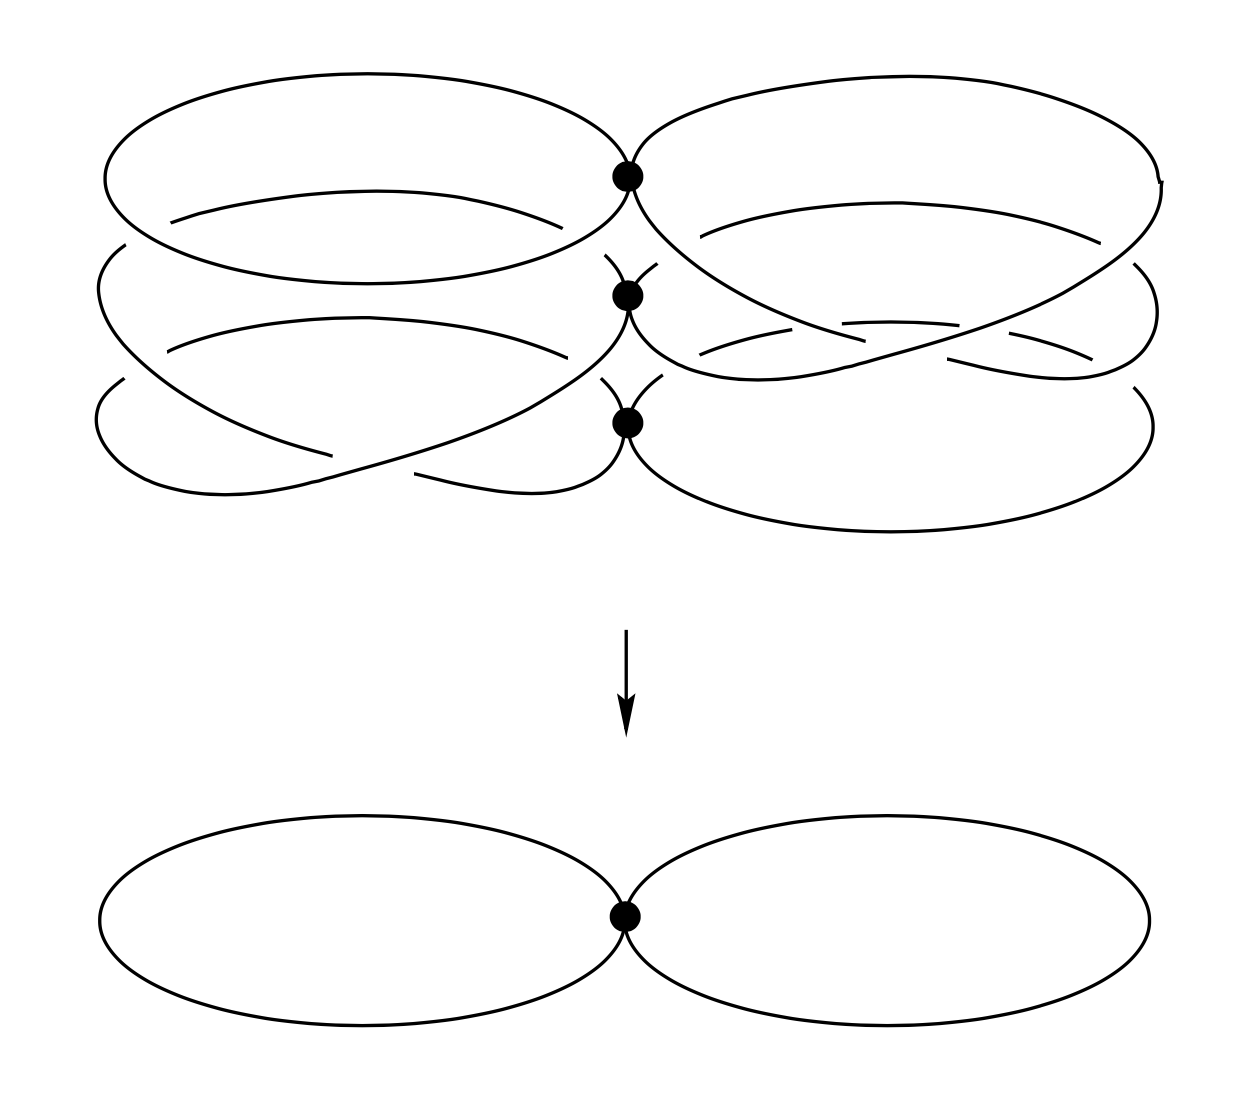
\includegraphics[width=1.5in]{fig12.9.png}
\end{center}

\begin{enumerate}[(a)]
\item Identify the subgroup $q_*\pi_1(X_4,1)\subseteq \pi_1(X_2,1)$ in terms of the generators described in Example 11.17.
\item Prove that $q$ is not a normal covering map.
\end{enumerate}
\end{prob}

\end{document}